\documentclass[12 pt]{article}
\usepackage{graphicx}
\usepackage{enumitem}
 \renewcommand{\baselinestretch}{1.5}
\usepackage[margin=.75 in]{geometry}

\usepackage{parskip}
\parindent=0
\usepackage{natbib}
\bibliographystyle{nature}

\title{Phenological differences among species explain why early leafout extends the calander but not thermal growing season}

\author{Dan, Cat, Deidre and Lizzie}
\begin{document}
\maketitle}
%\setlength{\parskip}{0.5pt} % 1ex plus 0.5ex minus 0.2ex}
\setlength{\parindent}{0}

\section{Introduction}
Carbon uptake by terrestrial plants is a major determinant of Earth's climate system \citep{} (say more precisely). In mid and high latitudes, the net carbon uptake is primarily determined by the length of the growing season \citep{}. Because climate change has advanced spring leafout, widely considered the start of the growing season \citep{} it has been suggested that earlier start of season should translate into a longer growing season and, therefore, more net carbon uptake by terrestrial ecosystems \citep{}. However we haven't really seen this in the data \citep{}. Quantifying carbon uptake by terrestrial plants is a critical aspect of climate forecasting, and therefore it is critical to understand the relationship between phenology, growing seasons and carbon storage.

One possible reason that earlier spring phenology many not increase net carbon assimilation (choose a term and stick with it) is if and early start of growing season results in an earlier end of the growing season. These phenological carryover effects (positive associates between phenological phases) are prevalent \citep{} but weaken over the season \citep{}, so it is unlikely variation in SoS and EoS are perfectly correlated, and this is reinforced by the observations that calendar growing seasons have indeed gotten longer with climate change.

But conditions that are suitable for photosynthesis are not uniform across the year (Figure 1a). While earlier leafout may increase the lent of the calendar growing season, such shifts may have little effect on the thermal growing season, defined here as....\citep{} because the early spring isn't favorable. The thermal growth season is likely a better proxy for carbon gain. Even with very weak carry-over effects between SoS and EoS, phenological advances that drive SoS into less favorable conditions for carbon assimilation in the early spring, trade more carbon gain in mid season for reduced gain in early. 

We can see these dynamics tracking the phenology of four individuals plants from the study we present below. The earlier individual of \emph{Aronia melanocarpa} depicted in Figure \ref{fig:concept}a, starts growing 24 days before a later individual, but only ceases 13 days before it (i.e., it has a 14 day longer calendar growing season). However, because the 24 day growth advantage it has occurs when thermal conditions are less favorable, it ends up having a shorter thermal growing season (i.e., less change for carbon assimilation) than its later nonspecific (Figure \ref{fig:concept}b). This is not the case for the later leafing species \emph{Myrica gale} where the both the earlier and later leafing individual start growing under more optimal thermal conditions, so the 20 day ``head start" the earlier individual incurs results in a both a longer calendar and thermal growing season (Figure \ref{fig:concept}a,c). 

These dynamics suggest that the carbon gain from an extended growing season, depends not only on the magnitude of phenological shifts but also the timing of those shifts relative to thermal conditions of the vegetative period, which not only vary across time and space, but also across the species that comprise forest communities. Understanding all this (say better) requires  understanding how the relationship between SoS and both thermal and calendar growing season varies depending on the unique phenological positions the species that make up a community. However, this is super difficult to do because...a few reason including...  

In this study, we use phenological observations from a multi-species common garden study to 
assess how variation in leafout and  budset phenological among species, years and populations affects the length of the calendar and thermal growing season. Specifically we ask:

\begin{enumerate}
\item How strong is the carry-over effect between leafout and budset? 
\item Which phase more strongly influence variation in growing season length across years, species and populations?
\item How does variation in the leafout affect the length of the thermal and calendar growing season?
\end{enumerate}

This study offers insights into physiology that will allow us to scale from ecosystem level observations to individual mechanisms woo, and improve forecasting.

\section{Methods}
\subsubsection{The common garden at Weld Hill}
In 2014-2015, we collected seeds of 18 species woody plants from four field sites in eastern Northern America spanning a Y degree latitudinal gradient. The four field sites included Harvard Forest (Lat long), the Second College Grant of Dartmouth College (lat long) White mountains (lat long) and St. Hippopotamus, CA (lat long). We transported all seed back the the Weld Hill Research Building at the Arnold Arboretum in Boston MA (lat long) where we germinated seeds following standard germination protocols, and grew them to seeding stages for a year or so in the research green house. In Spring of 2017 we planted them out to establish the common garden at Weld hill. Plantings were randomized between 16 plot blocks. Individuals that were to small to survive outside were maintained in the growth facilities for an additional year and out planted in the early spring of 2018 (i think). Plots were divided between tree plots which included species x,y,z and shrub plots which included species a,b,c,d and shade cloth. Plots were regularly weeded and watered throughout the duration of the study.

\subsubsection{Phenological monitoring:}
For the years of 2018-2019, we made phenological observations of all individuals in the common garden twice per week from February to December. In 2020 due to the COVID 19 pandemic we did it a bit less, but Cat can say how much. We describe phenological stages using a modified bbch scale \citep{} a common metrics for quantify woody plant phenological progression. We observed all major vegetative stages (budburst, bbch 07, leafout bbch 15, end of leaf expansion bbch 19, budset bbch X, and leaf coloration/drop bbch z, and reproductive phases flowering (60-65) and fruiting and fruit drop(). 

\subsubsection{Data analysis}
To better under the role that variation in leafout and budset phenology play in determine calendar growing season length among species populations and years we fit a Bayesian hierarchical with a Gaussian probability distribution. We calculated growing season duration by subtracting the day of leafout from the day of budset. We fit an intercept only model with phenophase timing (leafout, budset or growing season duration) as the response variable and partial pooling across species, populations and years. We only included observations with both budset and leafout observed on the same plant in this analysis (n= 595).

To assess the relationship between variation in leafout timing and calendar and thermal growing seasons we fit two additional regression models with thermal or calendar growing season length as the response variable and day of leafout as the main prediction. To account for species-level differences we included partially pooling on the slope and intercept of species.

We define the thermal growing season as the cumulative growing degree day heat sums between the day of leafout and the day of budset for each species. We calculated daily heat sums using the R package pollen \citep{} using a 10 $\degree$C base temperature with minimum and maximum daily temperature data from the weld hill weather station.

All models were fit in the R package brms on 4 chains with a 4000 iteration warm-up and 1000 sampling iterations on each chain for a total of 4,000 sampling iterations across all chains. We evaluated model fit, with no divergent transitions, rhats less than 1.01 and high effective sample sizes. All analysis were done in R.

\section{Results}
\subsubsection{Sources of variation in calander growing season}
There was high variance in leafout timing among species and years ($\sigma_{species}$: 8.23 $UI_{95}$[5.22,12.81], $\sigma_{year}$:10.49 $UI_{95}$[4.27,24.60], Figure \ref{fig:vapar}a,b). Population level variation was low ($\sigma_{population}$:0.62, $UI_{95}$[0.02,2.82], Figure \ref{fig:vapar}c). \emph{Sambucus racemosa} was typically the first species to leafout in the spring, leafing out approximately two weeks before \emph{Sorbus americana} the last species to leaf out (Figure \ref{fig:vapar}c). There were no differences in leafout timing among the four populations included in our study (Figure \ref{fig:vapar}c). Leafout was the earliest in 2019 and the latest in 2020 (Figure \ref{fig:vapar}c). 

Relative to leafout, variance in budset timing was higher for species, years and populations ($\sigma_{species}$: 9.81 $UI_{95}$[ 6.61,14.49], $\sigma_{year}$: 14.92 $UI_{95}$[5.68,9.21], $\sigma_{population}$: 2.35, $UI_{95}$[0.23,8.51], Figure \ref{fig:vapar}), but followed similar relative contributions (highest variance in year, lowest in population).
Budset was earliest for \emph{Amelanchier canadensis} and latest for \emph{Alnus incana} and \emph{Betula paperifera} with more than three weeks between them (Figure \ref{fig:vapar}a). Populations from the Second College Grant set buds approximately three days before those at the from the white mountains, but these differences statistically weak (Figure \ref{fig:vapar}b). Like leafout 2019 had the earliest budset and 2020 the latest (Figure \ref{fig:vapar}b).

Variance in growing season length was highest among species ($\sigma_{species}$: 14.38, $UI_{95}$[9.85,20.81] and lower among years ($\sigma_{year}$: 4.67 $UI_{95}$[0.76,8.63], Figure \ref{fig:vapar}b) and populations ($\sigma_{population}$: 2.50, $UI_{95}$[0.19,2.82], Figure \ref{fig:vapar}c). Due to it's early leafout and late budset \emph{S.racemosa} had the longest calendar growing season of the species in our study. \emph{A. canadensis} and \emph{S. americana} had the shortest growing seasons, though for \emph{A. canadensis} this was due to early budset and for \emph{S. americana} late leafout (Figure \ref{fig:vapar}a). Population level differences in calendar growing season were determined by differences in budset, and followed the same pattern with Grant marginally earliest and white mountains  latest, with high uncertainty. (Figure \ref{fig:vapar}b). Despite substantial difference among years for leafout and budset, the calender growing season remained consistent over the three year study period (Figure \ref{fig:vapar}c).

The lower levels of variance among year in growing season length we observed relative to the high variance in both leafout and budset indicate that variation in the SoS and EoS among years is positively associated (ie early leafout= earlier budset), which is supported by weak but positive pearsons correlation coefficient of 0.32 $CI_{95}$[0.25, 0.39] we found between leafout and budset in our study.

\subsubsection{Relationship between leafout phenology and calander and thermal growing seasons}

We found that later leafout resulted in a shorter calendar growing season (Figure \ref{fig:thermcal}a) and that this relationship was consistent across species, though varying strength  (Figure \ref{fig:thermcal}b).

In contrast, we found that a generally later leafout resulted in a longer thermal growing season (Figure \ref{fig:thermcal}c) in our study. This effect was stronger for species that typically leaf out earlier in the spring relative to others like \emph{Sambucus racemosa}, \emph{Viburnum cassiodes}, \emph{Spirea alba}, \emph{Diervella lonicera}, \emph{Aronia melanocarpa} \emph{Spirea tomentosa} and \emph{Betula populifolia} and was weaker in later species like \emph{Betula papyrifera}, \emph{Betula allegheniensis} and \emph{Alnus incana}(Figure \ref{fig:thermcal}d).


\section{Discussion}
Our multi-species common garden study showed that for already early leafing species, earlier leafout does not extend their thermal growing season---a proxy for potential carbon uptake period---despite extending the calendar growing season. In fact, we found that for these early leafing taxa, delayed leafout resulted in a longer thermal growing season. This relationship was in part explained by phenological carry-over between leafout and budset where later leafing individuals also set buds later, extending their growth into that later part of the season when thermal conditions were more favorable.  For later leafing species, earlier leafout did not substantially reduce their thermal growing season. This is likely because for them, even an earlier relative leafout still occurred in thermally favorable times of the season, and a relatively small advance in calendar time resulting in a proportionately large gain in thermal sums.

The dynamics may help to explain why phenology advances with climate change have not clearly translated into higher levels of primary productive \citep{}. Our results show that there is little advantage from a carbon or primary productive perspective for leafing out too early in the season, as thermal conditions are not favorable for photosynthesis and assimilation. Many of the species that are most phenologically sensitive to climate change are already among the earliest species to leaf out in temperate plant communities \citep{}, implying their may be little to gain from a carbon perspective.

So then why are species early? How is it then that phenologically trackers are doing better? \citep{}. In our study we only evaluated the thermal conditions that may affect photosynthesis, rather than photosynthesis itself, which also depends strongly on light availability which in forest systems is highly dependent on biotic interactions. In our study, the species that leafed out the earliest are under story shrubs, for whom access to light becomes severely limited later in the growing season as canopy trees leaf out. It may be that for these species, the light availability early in the season necessitates leafing out in thermally bad conditions. In fact, some studies suggest that under story shrubs get all/most of their carbon before canopy closure \citep{}.

The phenological carry-over effects between leafout and budset that we observed was interesting in light of the fact that spring phenological phases are reported to be more plastic than autumn ones (is this still true?). Some of this might have to do with scale of measurement---macro-scale measurements like remote sensing may detect different things. Budset is the end of primary growth which we observed closely   

The low levels of phenological variance between populations in our common garden provide little evidence for local adaptation in phenology. We found slightly stronger evidence for budset than leafout, which is consistent with the literature \citep{}. 

 This study shows linking phenological growing season to primary productivity requires account for phenological variation at multiple scales (individual, species level, multiple phases). Some forward thinking implications paragraph here.


\section{Figures}
\begin{figure}[h!]
    \centering
 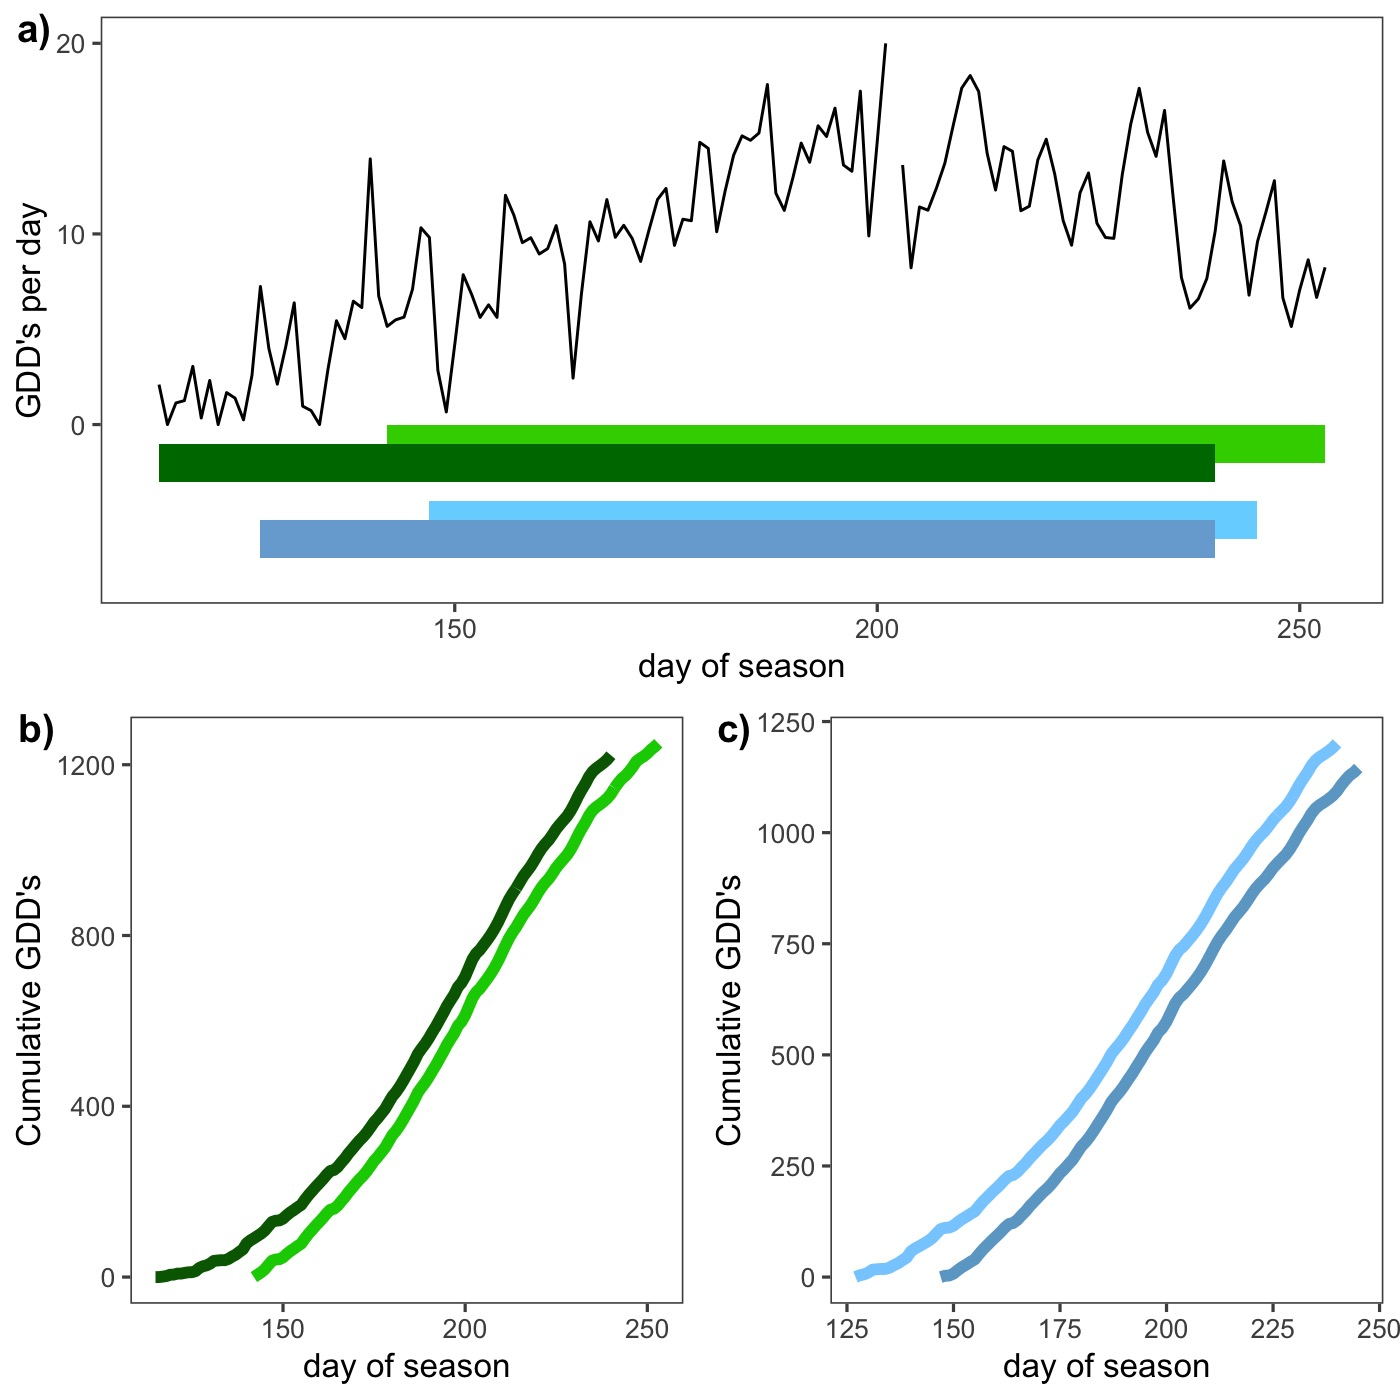
\includegraphics[width=.5\textwidth]{..//analyses/figures/aronia_examp.jpeg}
    \caption{Thermal conditions vary across the calendar growing season, which can generate a complex relationship between the calendar and thermal growing seasons. Panel a) depicts the daily heat sums at the Weld Hill Research Building in 2019 and the calendar growth season of early and late leafing individuals of \emph{Aronia melanocarpa} (green bars) and \emph{Myrica gale}(blue bars). Despite the fact the the early individual of \emph{A. melanocarpa} leafs out 24 days before it's later con-generic and only sets bud 13 days before it (i.e., it has a 14 day longer calendar growing season) it's thermal growing season is shorter (panel b) because most of its growth advantage (explain this better) takes place in the unfavorable early spring. In contrast for \emph{M. gale} where both the early and late individual leaf out later in the spring, the 20 day head start and 5 day earlier finish of the earlier individual (15 day longer calendar growing season) results in a longer thermal growing season for it as well (panel c)}.
    \label{fig:concept}
\end{figure}


\begin{figure}[h!]
    \centering
 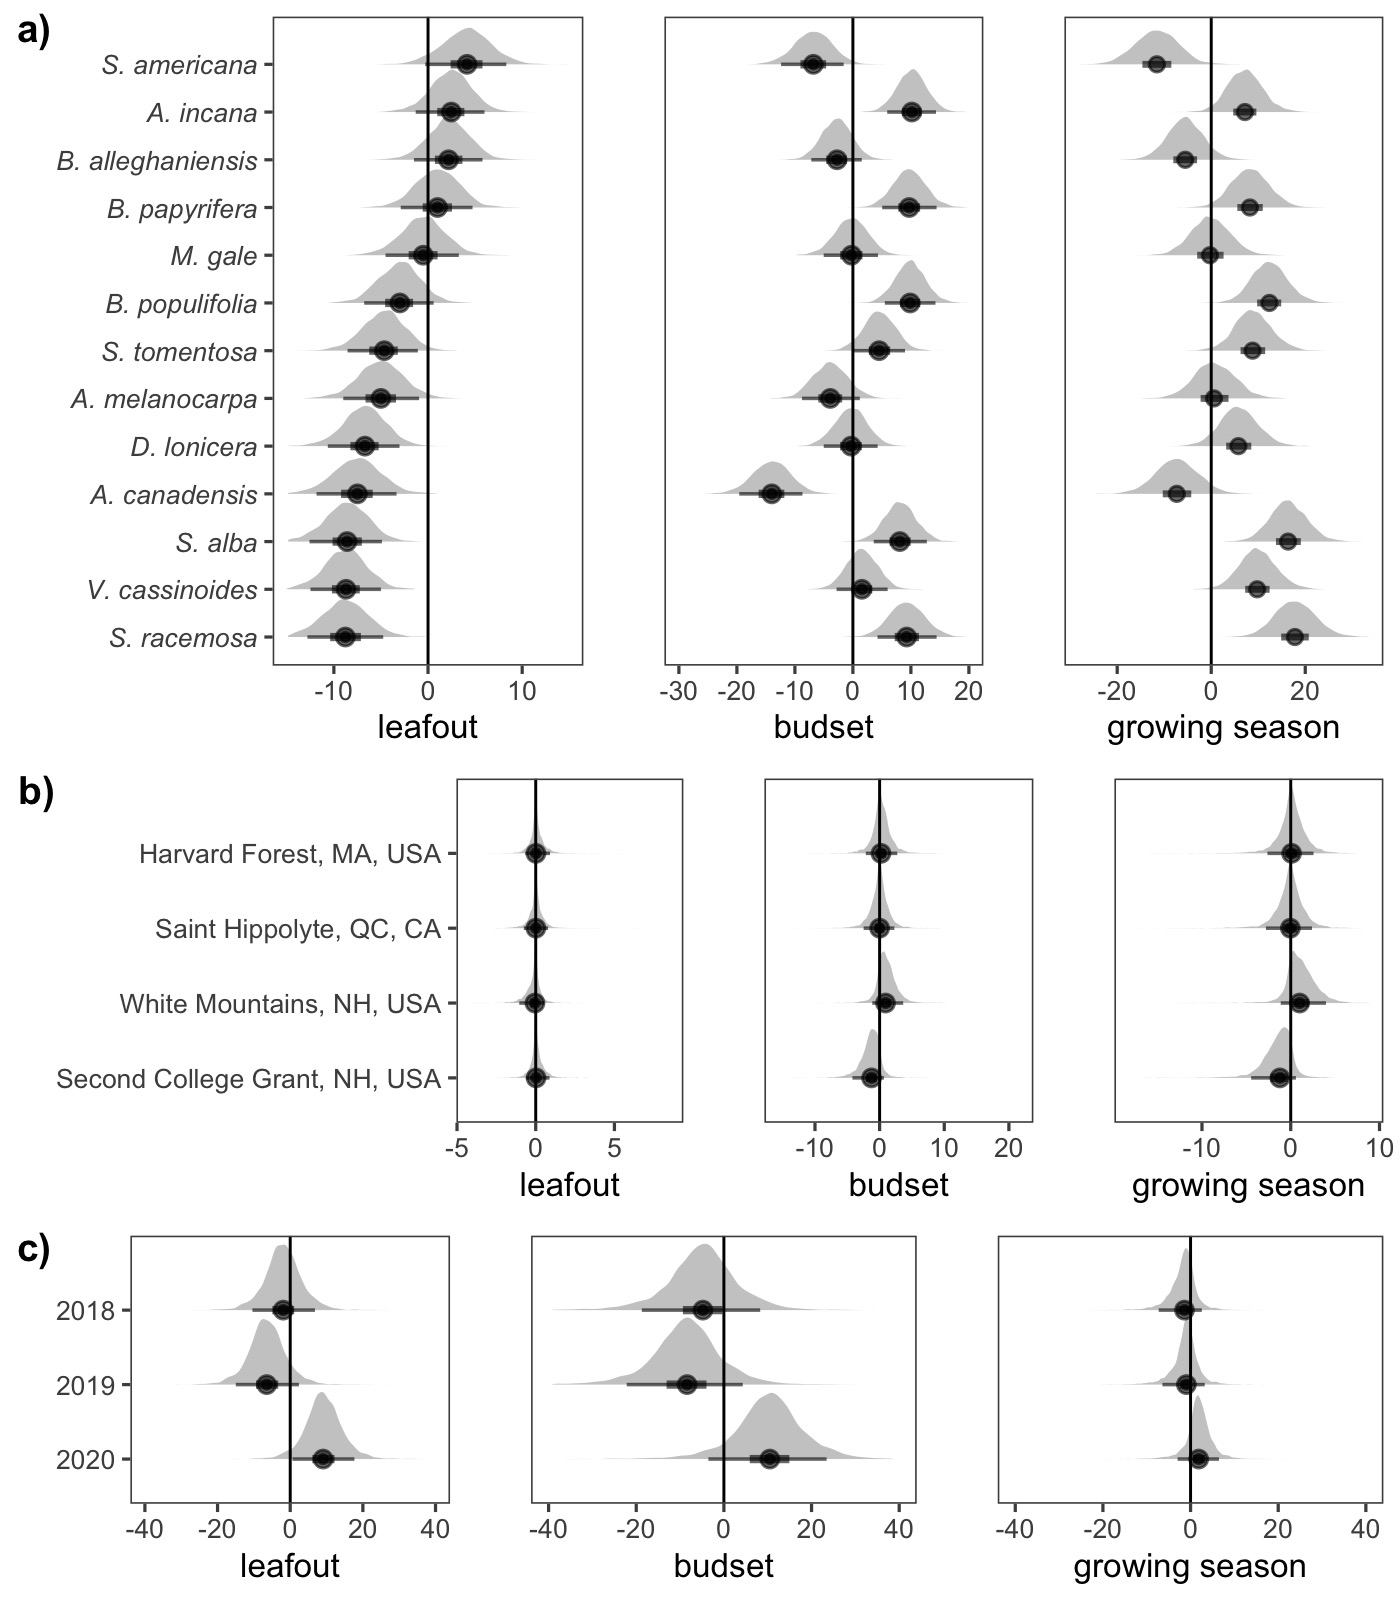
\includegraphics[width=.7\textwidth]{..//analyses/figures/var_parts.jpeg}
    \caption{Differenece in leafout, budset and calander growing season length partioned between species (a) populations (b) and years (c). Point represent the median effect size estimate, and bars the 50\% uncertainty intervials. The grey distribrion depict the full uncertaintly estiamte around the estimate.}
    \label{fig:vapar}
\end{figure}


\begin{figure}[h!]
    \centering
 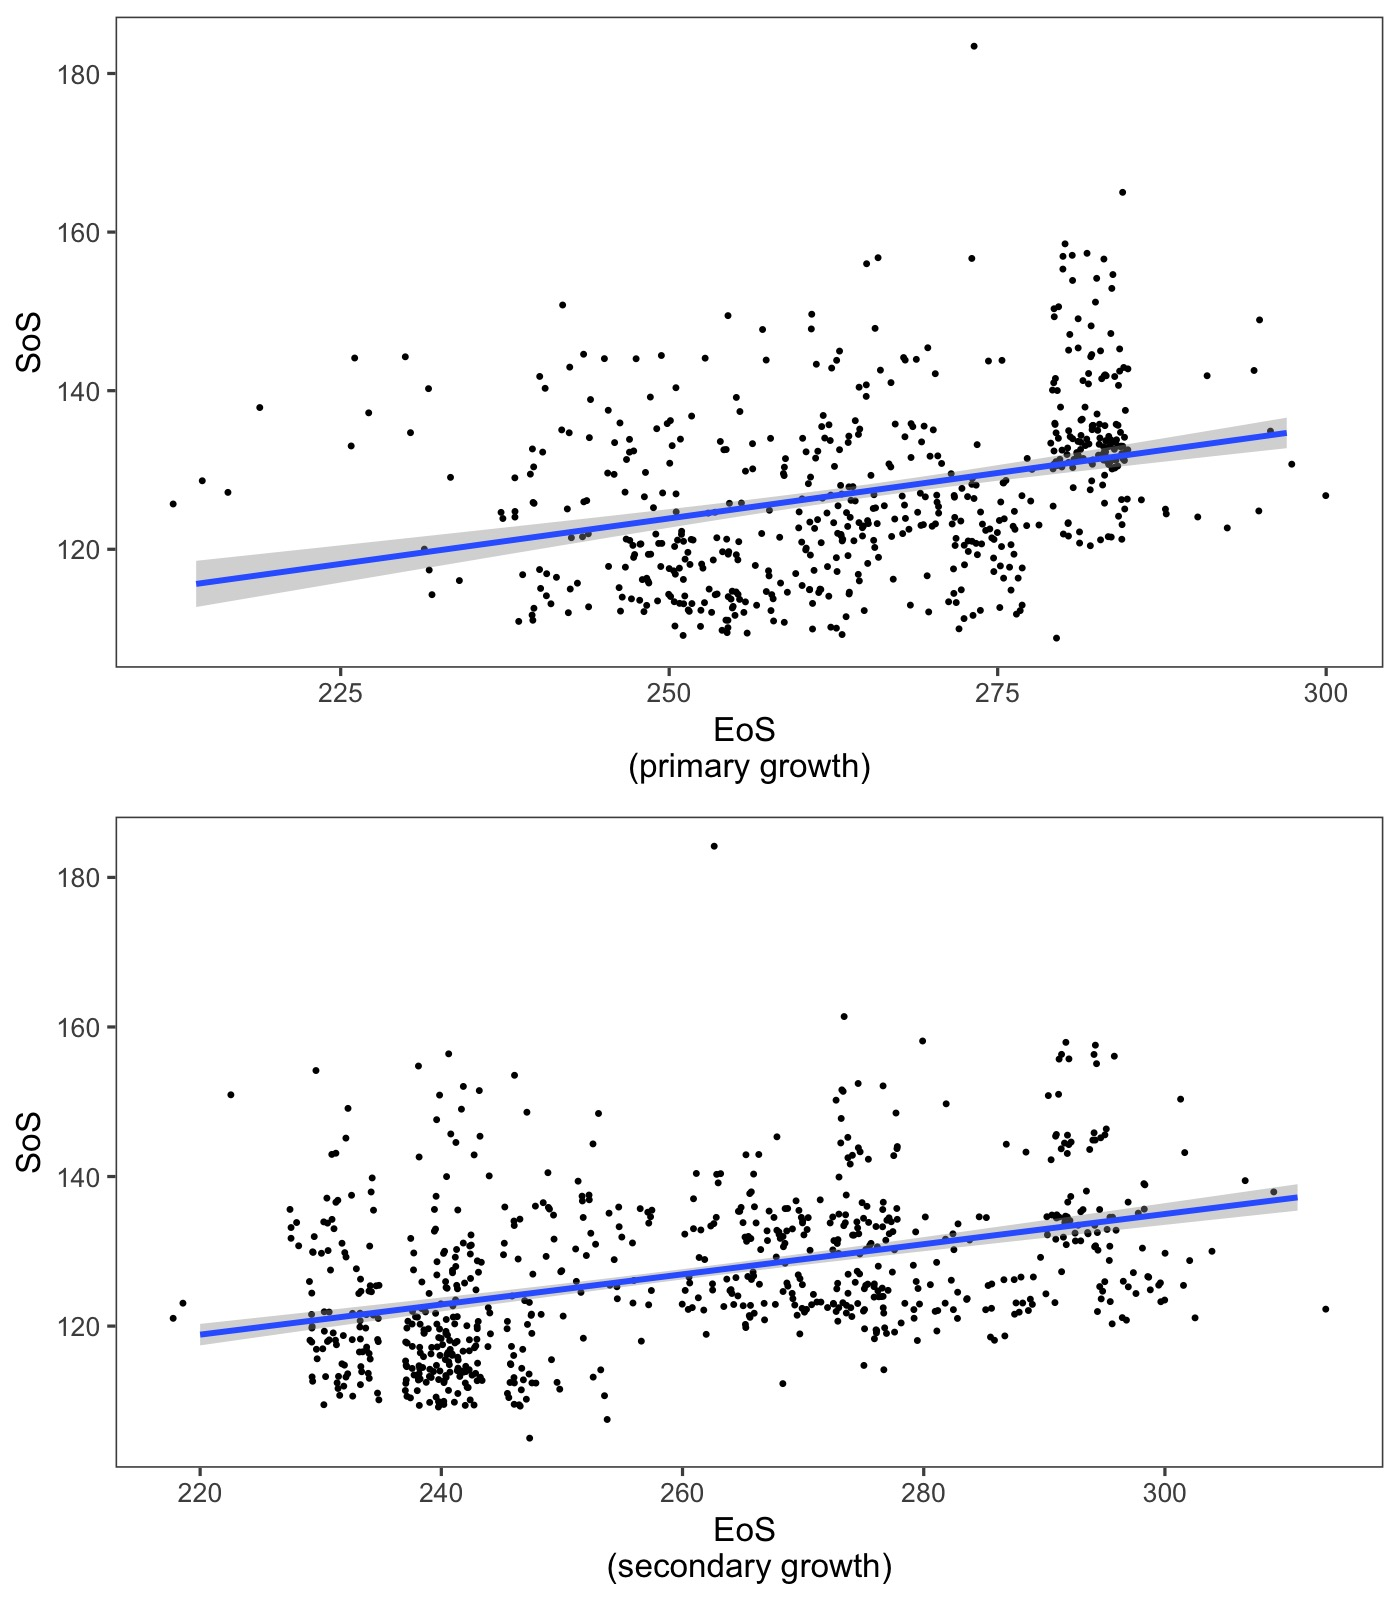
\includegraphics[width=.7\textwidth]{..//analyses/figures/primarygrowingseason_modplots.jpeg}
    \caption{The relationship between Start of Spring (SoS; calendar day of leafout) and growing season length differs between the calendar growing season and the thermal growing season. An increasing later SoS resulted in a shorter calendar growing season (panel a) and this pattern was consistent across species in our study (panel b). In contrast, an increasing later SoS resulted in a longer thermal growing season (panel c) though this effect was stronger for species that typically leafout earlier in the season---panels in c) are display in the typical order of leafout among species. The blue trend lines represent the mean effect of SoS timing on growing season length and black lines represent 1000 draws from the posterior distribution as a measure of uncertainty. Points in a), and c) represent the raw data. \textbf{to do: rename x-axis on b and d and write our the species names}}
    \label{fig:thermcal}
\end{figure}
\end{document}